

% This LaTeX was auto-generated from an M-file by MATLAB.
% To make changes, update the M-file and republish this document.

\documentclass{article}
\usepackage{graphicx}
\usepackage{color}
\usepackage{listings}
\usepackage[framed]{mcode}
\usepackage{fullpage}
\usepackage{amsmath}
\usepackage[utf8x]{inputenc}
\usepackage{import}
\usepackage{setspace}
\usepackage{hyperref}
\definecolor{lightgray}{gray}{0.5}
\setlength{\parindent}{0pt}

\begin{document}

    
    
%\section*{}


\title{BE 521: Homework 0 Questions\\{\normalsize Introduction}\\{\normalsize Spring 2021}}
\author{15 points}
\date{Due: Thursday 1/28/2021 11:59 PM}
\maketitle
\textbf{Objective:} Working with the IEEG Portal, basic matlab commands, publishing LaTeX


\section{Unit Activity (15 pts)}
The dataset \texttt{I521\_A0001\_D001} contains an example of multiunit human iEEG data recorded by Itzhak Fried and colleagues at UCLA using 40 micron platinum-iridium electrodes.
Whenever you get new and potentially unfamiliar data, you should always play around with it: plot it, zoom in and out, look at the shape of individual items of interest (here, the spikes). The spikes here
will be events appx. 5 ms in duration with amplitudes significantly greater than surrounding background signal.
\begin{enumerate}
 \item Using the time-series visualization functionality of the IEEG
 Portal find a single time-window containing 4 spikes (use a window width
 of 500 ms). The signal gain should be adjusted so that the spikes can be seen in entirety. Give a screenshot of the IEEG Portal containing the requested plot.  Remember to reference the LaTeX tutorial if you need help with how to do this in LaTeX. (2 pts)\\

Include screenshot:
\begin{lstlisting}
% 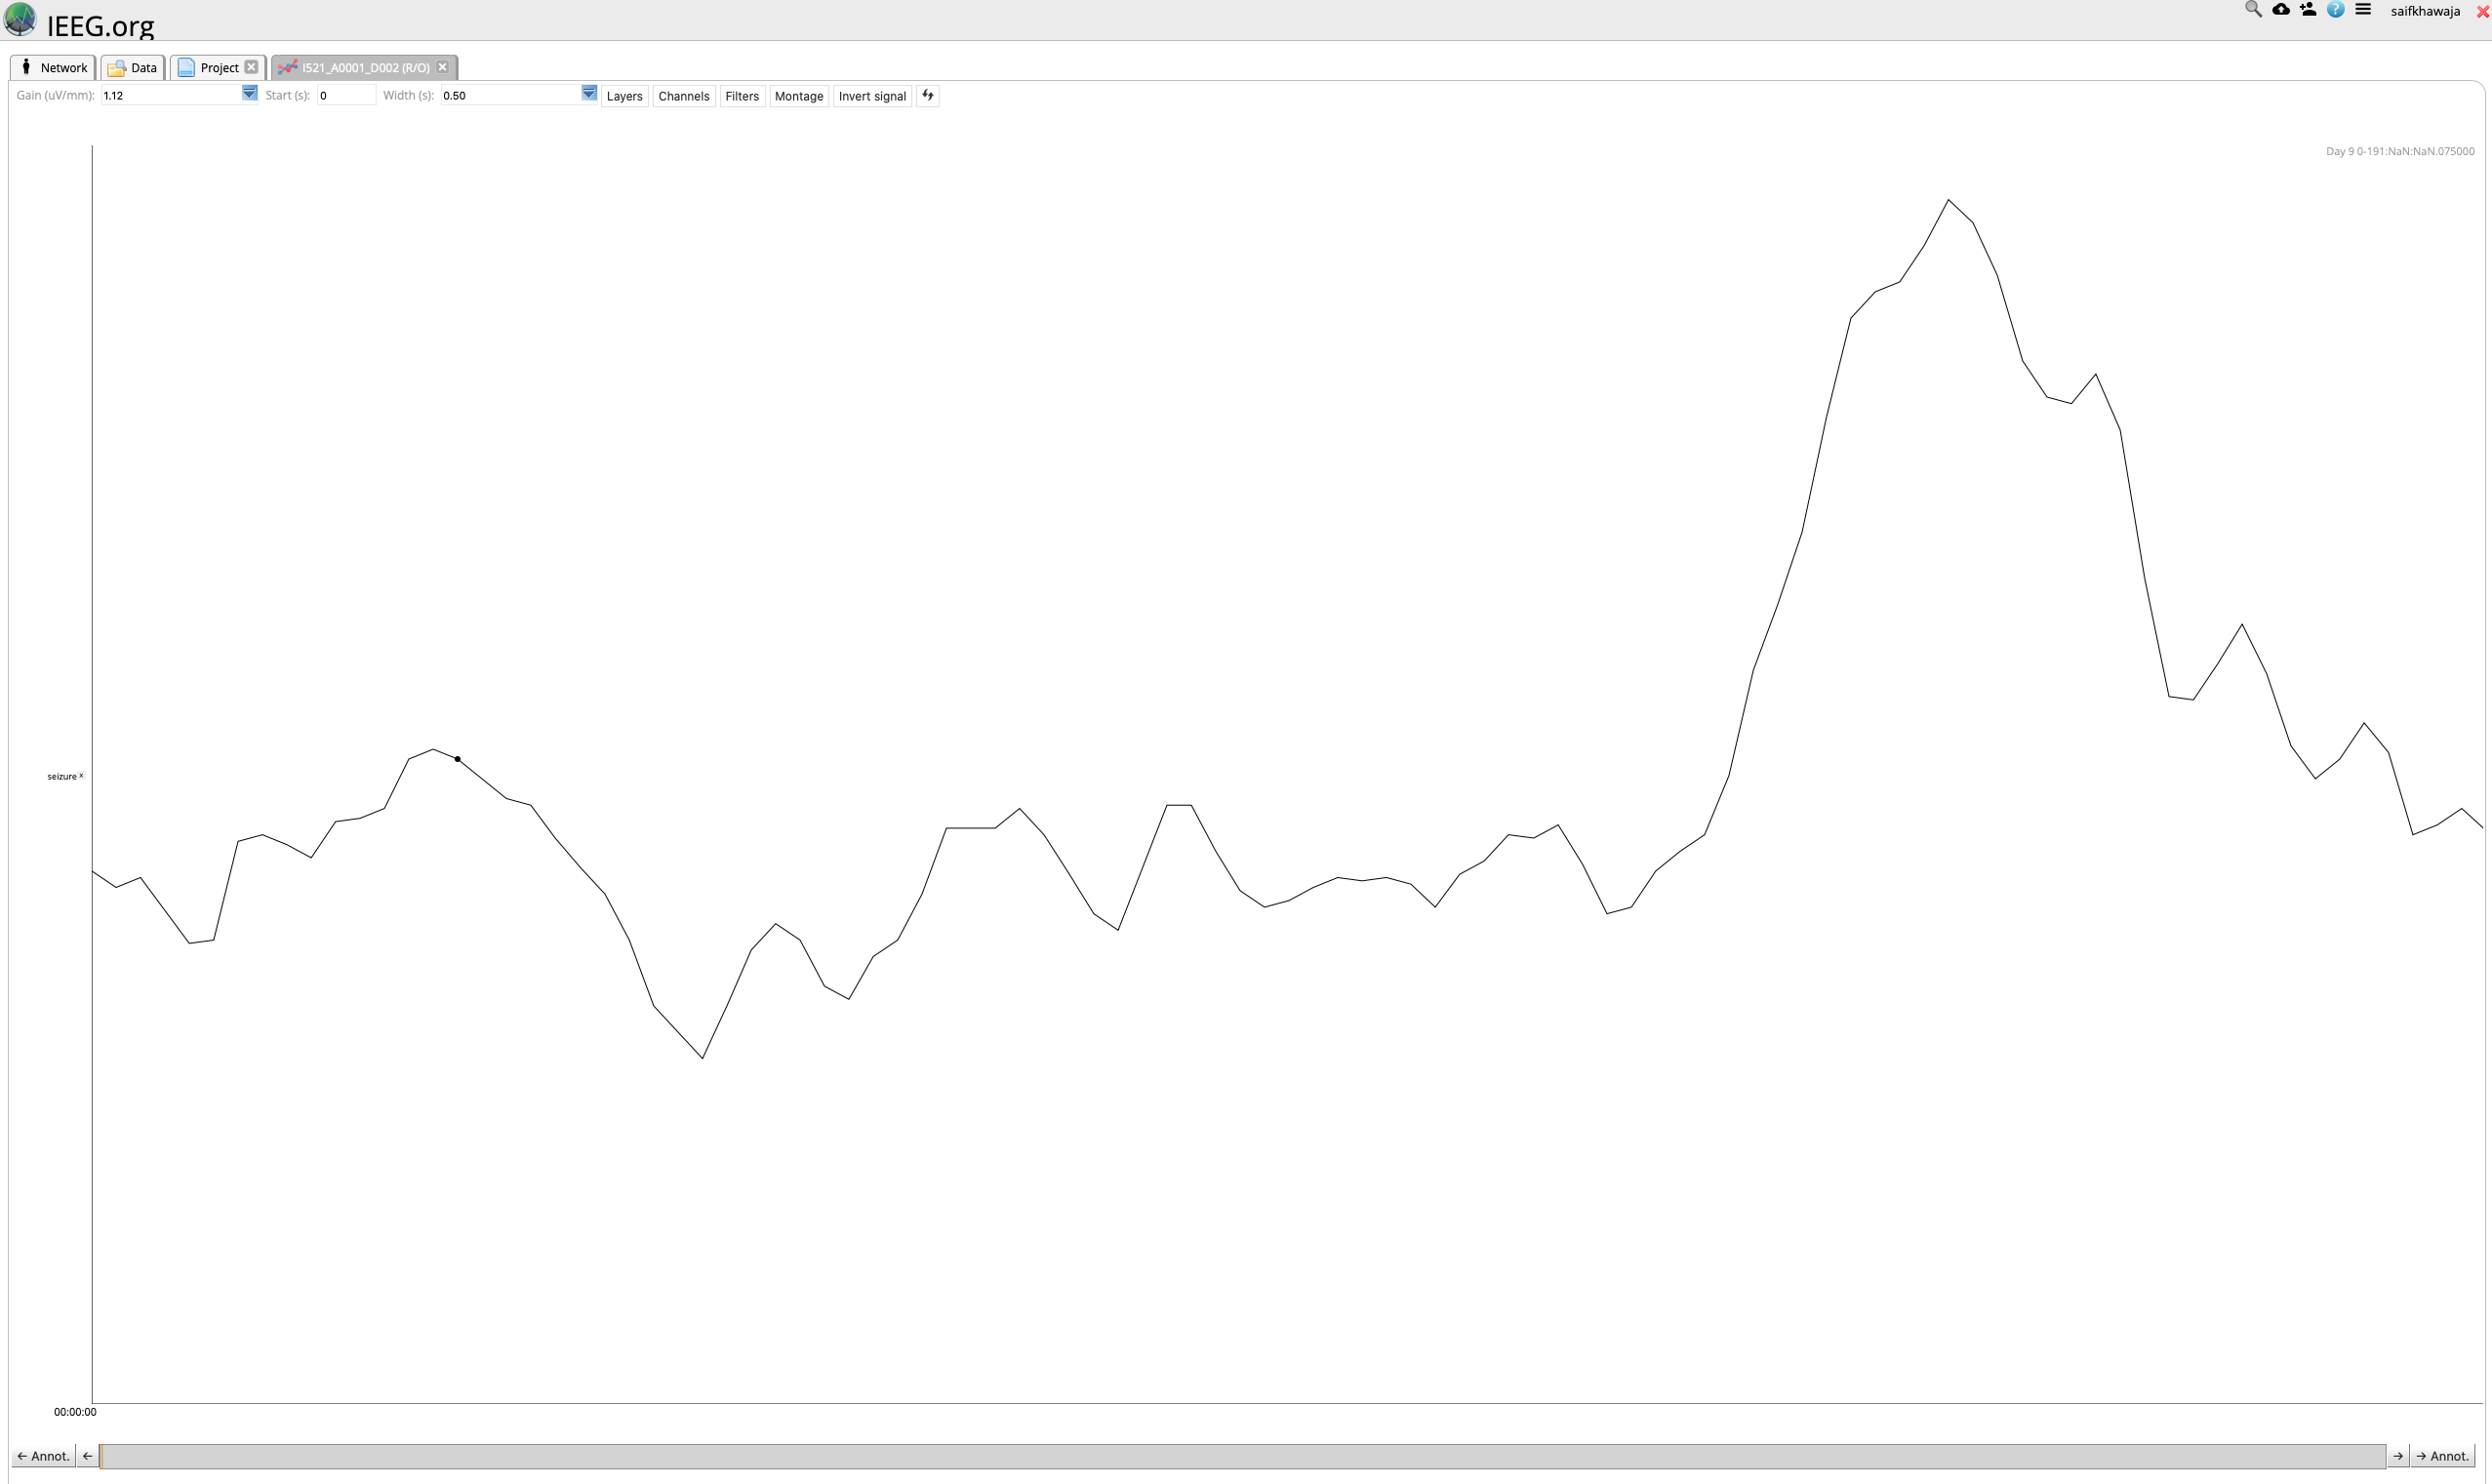
\includegraphics[scale=0.3]{/Users/saif/Documents/GitHub/braincomputerinterfaces/Homeworks/HW0/signal.png}\\
\end{lstlisting}

 \item Instantiate a new IEEGSession in MATLAB with the
 \texttt{I521\_A0001\_D001} dataset into a reference variable called
 \emph{session} (Hint: refer to the IEEGToolbox manual, class tutorial, or the built-in \emph{methods} commands in the \emph{IEEGSession} object - i.e., \emph{session.methods}). Print the output of \emph{session} here. (1 pt)\\

\begin{lstlisting}
% setup path

cd('/Users/saif/Documents/GitHub/braincomputerinterfaces/Homeworks');
addpath(genpath('ieeg-matlab-1.14.49'));
addpath(genpath('HW0'));
savepath;

% create access key

% yourPath = IEEGSession.createPwdFile('saifkhawaja','Saifkhawaja98!');

% create a session

session = IEEGSession('I521_A0001_D001', 'saifkhawaja', 'sai_ieeglogin.bin')
\end{lstlisting}

\color{lightgray} \begin{lstlisting}IEEGSETUP: Adding 'ieeg-matlab.jar' to dynamic classpath
Warning: Objects of edu/upenn/cis/db/mefview/services/TimeSeriesDetails class
exist - not clearing java 
Warning: Objects of edu/upenn/cis/db/mefview/services/TimeSeriesInterface class
exist - not clearing java 
IEEGSETUP: Found log4j on Java classpath.
URL: https://www.ieeg.org/services
Client user: saifkhawaja
Client password: ****

session = 

  <a href="matlab:help('IEEGSession')">IEEGSession</a>:

      server: 'ieeg.org'
    userName: 'saifkhawaja'
        data: [1x1 IEEGDataset]

  <a href="matlab:methods(IEEGSession)">Methods</a>, <a href="matlab:IEEGObject.openPortalSite()">main.ieeg.org</a>

\end{lstlisting} \color{black}

 \item What is the sampling rate of the recording? You can find this
 information by exploring the fields in the \emph{session} data structure
 you generated above. Give your answer in Hz. (2 pts)\\

\begin{lstlisting}
Hz = session.data.sampleRate
\end{lstlisting}

\color{lightgray} \begin{lstlisting}
Hz =

       32051

\end{lstlisting} \color{black}

 \item How long (in seconds) is this recording? (1 pt)\\

\begin{lstlisting}
% Obtain the duration of the recording for channel 1 (retuyrned in microseconds).

durationInUSec = session.data(1).rawChannels(1).get_tsdetails.getDuration;

% convert to seconds and return value
durationInSec = durationInUSec / 1e6
\end{lstlisting}

\color{lightgray} \begin{lstlisting}
durationInSec =

    10

\end{lstlisting} \color{black}

 \item
 \begin{enumerate}
    \item Using the \emph{session.data.getvalues} method retrieve the
    data from the time-window you plotted in Q1.1 and re-plot this data
    using MATLAB's plotting functionality. Note that the amplitude of the EEG signals from the portal is measured in units of $\mu V$ (microvolts), so label your y-axis accordingly.
    (NOTE: Always make sure to include the correct units and labels in your plots. This goes for the rest of this and all subsequent homeworks.). (3 pts)\\

\begin{lstlisting}
start_time = 6.08;
window_size = 0.5;
my_channel = 1;
dataWin = session.data.getvalues(start_time * 1e6, window_size * 1e6, my_channel);

figure();
plot(start_time:1/Hz:start_time + window_size, dataWin);
ylabel('\mu V');
xlabel('Time (seconds)');
title('Multi-unit Signal');
\end{lstlisting}


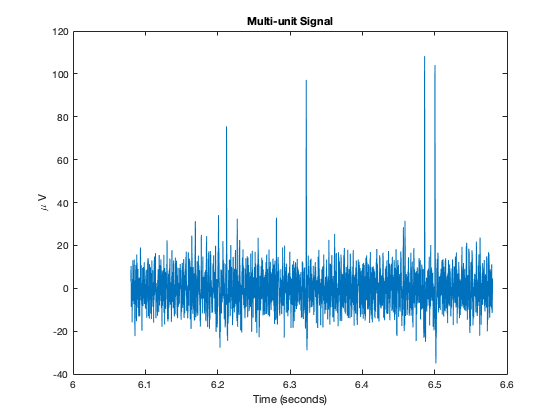
\includegraphics [width=5in]{HW0_Questions_01.png}

	\item Write a short bit of code to detect the times of each spike peak
	(i.e., the time of the maximum spike amplitude) within your
	time-window. Plot an 'x' above each spike peak that you detected superimposed on the plot from Q1.5a. (Hint: find where the slope of the signal changes from positive to negative and the signal is also above threshold.) (4 pts)\\

\begin{lstlisting}
thresh = 70;

inds_dF2 = diff( diff(dataWin) < 0 );
inds_thresh = dataWin(2:end-1) > thresh;
inds = find(inds_dF2 .* inds_thresh);

figure();
plot(start_time:(1/Hz):(start_time + window_size), dataWin);
ylabel('\mu V');
xlabel('Time (seconds)');
title('Multi-unit Signal');
\end{lstlisting}


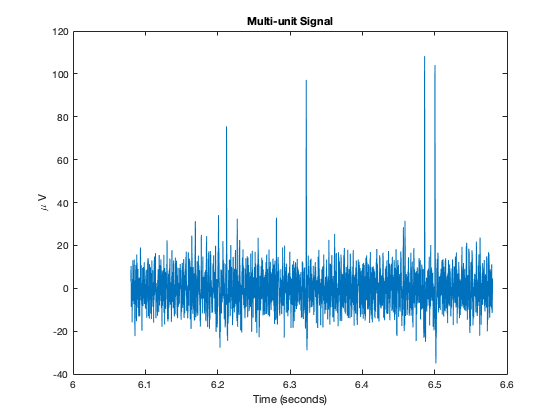
\includegraphics [width=5in]{HW0_Questions_02.png}

	\item How many spikes do you detect in the entire data sample? (1 pt)\\

\begin{lstlisting}
data = session.data.getvalues(1, 10*1e6, my_channel);

inds_dF2 = diff( diff(data) < 0 );
inds_thresh = data(2:end-1) > thresh;
inds = find(inds_dF2 .* inds_thresh);
N_spikes = length(inds)
\end{lstlisting}

\color{lightgray} \begin{lstlisting}
N_spikes =

    30

\end{lstlisting} \color{black}

\end{enumerate}
	\item Content Question- In the assigned reading, you
  learned about different methods to obtain and localize neural signals for BCIs.
  Describe the naming convention for the International 10-20 system for EEG recording. In your own words, what do the
	letters refer to and what can you infer from the parity (even vs. odd)
	of the number at a given site? (1 pt)\\

\begin{lstlisting}
% The 10-20 system uses electrodes positioned at 10, 20, 20, 20, 20 and 10%
% of total nsion-inion distances. This is so the distances between
% electrodes are uniform. The labels of the sites use letters that denote
% individual brain regions where they are located. From the parity, we can
% infer the indexing of both the transverse and antero-posterior
% placement.
\end{lstlisting}

\end{enumerate}




\end{document}
    
